% Generated from 05-机器人学的物理、控制与状态估计基础.md; edit the LaTeX source after migration.

\reportpart{第五部分 机器人学的物理、控制与状态估计基础}
\addcontentsline{toc}{part}{第五部分 机器人学的物理、控制与状态估计基础}
\markboth{第五部分 机器人学的物理、控制与状态估计基础}{第五部分 机器人学的物理、控制与状态估计基础}

前四部分已经建立了本报告的问题定义、历史主线和比较坐标。本部分的任务，则是把这些讨论压回机器人系统最难绕开的底层事实上：具身系统最终仍然要在一个受几何、动力学、接触、实时性和不确定性共同约束的物理世界中运行。无论后续采用的是模块化架构、学习型策略、VLA，还是更激进的统一基础模型路线，只要系统要真正进入物理闭环，就必须面对这里讨论的对象。

因此，本部分并不试图把传统机器人学教材完整重讲一遍，而是只聚焦那些在大模型时代仍然直接决定能力上限的基础：几何与状态表示、动力学与接触、规划与控制接口，以及状态估计与环境表征。这些内容不是“旧知识背景板”，而是后续所有现代具身系统仍然必须借用、改写或显式绕开的底层接口语言。以 \href{https://modernrobotics.org/}{《Modern Robotics》课程主页} 为代表的经典课程，至今仍把刚体运动、运动学、动力学、轨迹生成、运动规划和控制组织成同一条系统链条，这本身就说明这些问题并未被新的模型范式取消，只是被重新嵌入了新的系统中。

\section*{21. 刚体运动学与位姿表示}
\addcontentsline{toc}{chapter}{21. 刚体运动学与位姿表示}
\markboth{21. 刚体运动学与位姿表示}{21. 刚体运动学与位姿表示}

\subsection*{21.1 坐标系、齐次变换与旋转表示}
\addcontentsline{toc}{section}{21.1 坐标系、齐次变换与旋转表示}


机器人系统首先要回答的问题，并不是“如何推理”，而是“系统如何在数学上表达身体与世界的位置关系”。只要系统需要感知环境、规划动作、执行控制，就必然需要一种统一方式来表示刚体位姿、坐标变换和参考系关系。若这一步表述不清，那么后续关于目标位姿、误差、约束和运动接口的全部讨论都会失去可计算基础。

在现代机器人学中，最常用的位姿表达之一是齐次变换矩阵：

\begingroup
\footnotesize
\begin{equation*}
T =
\begin{bmatrix}
R & p \\
0 & 1
\end{bmatrix}
\in SE(3)
\end{equation*}
\endgroup

其中，\(R \in SO(3)\) 表示旋转，\(p \in \mathbb{R}^3\) 表示平移。这个写法的重要性不在于形式优雅，而在于它允许我们用同一对象描述“一个坐标系相对于另一个坐标系的刚体变换”，从而把感知、规划和控制统一到同一套几何语言中。\href{https://modernrobotics.org/}{《Modern Robotics》课程主页} 对 \(SE(3)\)、刚体运动和构型空间的系统组织，也正说明位姿表示并不是预备知识，而是机器人系统接口的基础语言。

对旋转本身，常见表示包括欧拉角、旋转矩阵和四元数。欧拉角的优点是直观，但存在奇异性；旋转矩阵无奇异性且便于组合，但参数冗余；四元数参数更紧凑，数值性质较好，因而在状态估计、轨迹插值和姿态控制中经常被优先使用。这里最重要的判断不是“哪一种表示绝对最好”，而是不同表示适合不同系统接口：例如，规划和推导时常用旋转矩阵或指数坐标，状态估计与插值时常用四元数，工程调试和可视化中则可能仍会回到欧拉角。

在具身智能讨论中，这一点经常被低估。因为当人们把系统能力主要表述为“语言到动作”或“图像到动作”时，很容易忽略动作输出最终仍然要投影到具体位姿、速度、关节状态和误差定义上。也就是说，高层表示可以更语义化，但底层物理接口并不会凭空消失。

\subsection*{21.2 欧拉角、旋转矩阵、四元数的比较}
\addcontentsline{toc}{section}{21.2 欧拉角、旋转矩阵、四元数的比较}


这三种表示的差异，不应只理解为“数学形式不同”，而应理解为它们分别在参数紧凑性、数值稳定性、几何直观性和计算便利性上做了不同取舍。欧拉角最直观，适合人类理解姿态与局部约束，但存在万向节锁与局部不连续问题；旋转矩阵表达冗余却全局一致，适合组合变换和刚体运动推导；四元数在插值、优化与姿态跟踪中常更稳定，但对初学者不够直观。

对现代具身系统而言，这种比较的价值不在于选择唯一“最先进”的表示，而在于理解不同模块为何偏爱不同形式。感知与状态估计模块可能更常在矩阵和四元数空间工作，界面展示或任务约束层可能仍使用欧拉角语言，而优化与控制层则更关注哪一种表示在迭代和约束处理中最稳。

从工程角度看，三种表示各有典型失效模式。欧拉角虽然直观，却容易在 pitch 接近特定角度时出现 gimbal lock；旋转矩阵保持了群结构和数值稳定性，但必须满足正交约束；四元数虽然适合连续姿态表示和球面插值，却需要保持单位范数，并且在符号上存在双覆盖问题。

如果把这些差异写成系统设计选择，那么它们本质上是在不同接口处做折中：

\begin{enumerate}
\item 人类可读性与控制可计算性之间的折中
\item 参数紧凑性与约束处理复杂度之间的折中
\item 局部线性化便利性与全局无奇异性之间的折中
\end{enumerate}

这类折中在后文也会反复出现。许多现代模型之所以看起来“直接输出动作”，只是因为中间几何层被隐藏了，而不是因为几何问题不再存在。

\subsection*{21.3 速度、加速度与雅可比矩阵}
\addcontentsline{toc}{section}{21.3 速度、加速度与雅可比矩阵}


如果把这一节只理解成“一个把关节速度映射到末端速度的矩阵工具”，会低估它在现代具身系统里的地位。雅可比矩阵本质上定义了局部可行动作空间的几何形状：哪些任务空间方向容易实现，哪些方向接近奇异，哪些方向会在关节空间中放大成高代价动作。也正因如此，很多看似属于高层策略的问题，最终都会在这一层暴露为可执行性问题。一个语言模型可以输出“向左轻推再抬起”的动作意图，但如果当前构型下该方向的雅可比条件数很差，低层系统就必须改写执行路径，甚至回退到重新选取抓取位姿。

位姿只描述“在哪里”，还不能描述“如何运动”。一旦系统进入轨迹跟踪、接触调节、视觉伺服或全身控制，就必须引入速度、加速度和任务空间与关节空间之间的映射关系。这里最关键的对象是雅可比矩阵：

\begin{equation*}
\dot{x} = J(q)\dot{q}
\end{equation*}

其中，\texttt{\detokenize{q}} 是关节变量，\(\dot{q}\) 是关节速度，\(\dot{x}\) 是末端执行器在任务空间中的 twist 或速度表示。这个公式的重要性在于，它把“高层想让末端怎么动”和“低层各个关节需要怎么动”连接起来。几乎所有现代操作系统、视觉伺服系统、阻抗控制器和全身控制器，都会在某种形式上使用这一映射。

进一步地，二阶关系会引出：

\begin{equation*}
\ddot{x} = J(q)\ddot{q} + \dot{J}(q,\dot{q})\dot{q}
\end{equation*}

这说明任务空间加速度并不只是关节加速度的简单线性映射，系统还必须处理由姿态变化引入的耦合项。这也是为什么很多看似简单的“末端到目标点”动作，在高速、强接触或多自由度系统中会迅速变得复杂。

\subsection*{21.4 为什么这些表示仍然是现代具身系统的底层语言}
\addcontentsline{toc}{section}{21.4 为什么这些表示仍然是现代具身系统的底层语言}


在大模型时代，最容易出现的一种误读，是把几何表示看成“旧时代的手工特征”。但从系统角度看，\(SE(3)\)、雅可比、任务空间误差和配置空间根本不是可以被轻易替代的“表示选择”，而是具身系统对物理世界进行可计算交互的最小语言。\href{https://lavalle.pl/planning/}{《Planning Algorithms》} 对构型空间、几何规划和带微分约束的规划所做的系统组织，进一步说明几何语言并不只用于推导教科书例题，而是直接决定规划与控制问题怎样被表述。

本节对后文最重要的意义，在于把“表示”重新放回接口位置。后文无论讨论 VLA 的动作 token、技能调用接口，还是世界模型中的 latent state，都必须面对一个事实：只要系统最终要进入真实物理执行链路，就必须在某处与这些经典几何对象发生映射关系。

\begin{lstlisting}[language=python]
# 示例：用任务空间速度目标通过雅可比伪逆求关节速度
import numpy as np

def joint_velocity_from_task_velocity(J, xdot, damping=1e-4):
    jj_t = J @ J.T
    damped_inv = np.linalg.inv(jj_t + damping * np.eye(jj_t.shape[0]))
    return J.T @ damped_inv @ xdot
\end{lstlisting}

上面的代码片段很简单，但它揭示了一个核心事实：即使高层目标来自语言或视觉模型，真正落到执行层时，系统仍然要通过类似这样的几何接口把任务空间目标映射到关节空间。

\section*{22. 机器人动力学与接触建模}
\addcontentsline{toc}{chapter}{22. 机器人动力学与接触建模}
\markboth{22. 机器人动力学与接触建模}{22. 机器人动力学与接触建模}

\subsection*{22.1 正逆动力学}
\addcontentsline{toc}{section}{22.1 正逆动力学}


从求解角度看，正动力学与逆动力学服务的是两类不同的问题。逆动力学更接近“为了跟踪给定轨迹，需要施加多大力矩”；正动力学则更接近“在当前力矩与外力条件下，系统会实际如何演化”。前者常被用在计算力矩控制、前馈补偿和模型预测控制中，后者则更接近仿真器、可达性分析和接触后果评估的基础接口。对具身系统而言，这一区分很重要，因为很多高层模型默认自己在输出“目标动作”，但工程系统真正需要的往往是可被逆动力学兑现、且其结果能被正动力学稳定验证的动作命令。

如果运动学回答的是“几何上怎么动”，动力学回答的则是“物理上能不能这样动，以及代价是什么”。机器人动力学的典型形式可写为：

\begingroup
\scriptsize
\begin{equation*}
M(q)\ddot{q} + C(q,\dot{q})\dot{q} + g(q) + \tau_{\mathrm{fric}} = \tau + J^T(q)F_{\mathrm{ext}}
\end{equation*}
\endgroup

其中，\(M(q)\) 是惯性矩阵，\(C(q,\dot{q})\) 表示科氏与离心项，\(g(q)\) 是重力项，\(\tau\) 是关节驱动力矩，\(F_{\mathrm{ext}}\) 是外部接触力。这个表达式之所以重要，是因为它把轨迹、控制输入、接触和系统响应统一放进了同一个物理约束框架中。

在真实系统中，动力学并不只是理论推导对象，而直接决定执行器选型、能耗上限、可实现加速度、负载边界和控制器设计空间。尤其当系统从桌面抓取走向双臂协同、全身运动、足式动态平衡和高动态操作时，忽略动力学代价通常会迅速转化为过热、失稳、振荡或接触失败。

\subsection*{22.2 刚柔耦合与接触动力学}
\addcontentsline{toc}{section}{22.2 刚柔耦合与接触动力学}


具身系统真正困难的部分，往往不是自由空间中的移动，而是接触发生之后的行为。接触问题之所以棘手，在于系统一旦接触环境，就不再只是在低维轨迹空间中移动，而是在一个受摩擦、顺应性、接触不确定性和混合约束共同控制的系统中演化。Hogan 关于阻抗控制的经典工作 \href{https://locomotion.csail.mit.edu/elib.cgi?b=Hogan85b}{《Impedance Control: An Approach to Manipulation, Part I》} 之所以长期重要，正是因为它正面回答了“系统如何在接触时表现出合适的动态关系，而不只是死板地跟踪位置命令”这一问题。

接触过程中的核心矛盾之一，是系统既要足够刚，以保证任务精度，又要足够柔顺，以吸收环境不确定性。位置控制如果过硬，在插接、装配、擦拭、推门或抓取柔性对象时很容易引发冲击与卡死；完全被动力量控制则又可能丧失任务几何精度。因此，很多现实系统采用的并不是简单的“位置控制”或“力控制”二选一，而是更丰富的混合力位控制、阻抗控制、顺应控制和 operational space control。

从系统建模角度看，接触之所以困难，还在于它通常把系统从单一光滑动力学切换成了带模式跳变的混合系统。未接触时是一套动力学，接触发生后约束集合与有效自由度都会改变，摩擦锥、接触法向和局部柔顺性也会立刻进入闭环。因此，很多在自由空间中表现稳定的轨迹与控制器，一旦进入接触阶段就会迅速暴露出过冲、振荡或卡滞问题。

\subsection*{22.3 力/位混合控制问题}
\addcontentsline{toc}{section}{22.3 力/位混合控制问题}


力/位混合控制的基本思想是：沿某些方向精确约束位置，沿另一些方向调节力或阻抗。例如，在平面擦拭任务中，法向需要维持合适接触力，而切向则需要跟踪目标运动轨迹。Khatib 提出的任务空间表述框架，以及后续任务空间控制路线，都在试图把这种需求写成更自然的控制接口：系统不只是跟踪关节量，而是在任务空间中调节与环境交互的行为，相关原始论文可参见 \href{https://khatib.stanford.edu/publications/pdfs/Khatib_1987_RA.pdf}{《The Operational Space Formulation》}。

一个简单的阻抗控制形式可以写成：

\begingroup
\footnotesize
\begin{equation*}
F = K(x_d - x) + D(\dot{x}_d - \dot{x}) + M(\ddot{x}_d - \ddot{x})
\end{equation*}
\endgroup

其中，\texttt{\detokenize{K}}、\texttt{\detokenize{D}}、\texttt{\detokenize{M}} 分别控制期望的刚度、阻尼和惯性行为。这个式子之所以重要，不是因为它能概括所有接触控制，而是因为它体现了一种根本思想：在接触任务中，系统需要控制的往往不是单个位置误差，而是与环境相互作用时表现出的动态关系。

\subsection*{22.4 为什么接触问题不会被“更大模型”自动抹平}
\addcontentsline{toc}{section}{22.4 为什么接触问题不会被“更大模型”自动抹平}


接触问题之所以不会被更大模型自动抹平，是因为它牵涉的不只是识别精度，而是高敏感、强非线性、局部突变且高度依赖具体身体结构的物理过程。接触一旦发生，力的传递、摩擦方向、材料顺应性、局部几何偏差和执行器延迟都会立刻进入闭环，而这些因素并不会因为模型“更懂语义”就自然变得可控。

更大的模型当然可以帮助系统更好地理解任务、对象和先验，但它并不能取消接触中的物理不连续性。真正有效的路径通常是把高层模型能力与触觉、力控、顺应控制、局部策略恢复和本体设计一同考虑，而不是期待参数规模单独解决执行现实。

当前很多具身智能演示主要聚焦视觉理解和高层任务接口，这容易让人产生一种错觉：只要模型更大、语义更强，接触问题迟早会自然解决。现实并非如此。越接近高精度装配、灵巧操作、全身接触和危险环境作业，系统越无法绕开执行器动态边界、末端顺应性、力反馈质量和接触不确定性。模型可以帮助系统更好地选择接触策略、预测任务阶段或调用技能，但它并不能取消接触本身的物理结构。

这也是为什么后文讨论 VLA、世界模型或技能调用时，不能把“动作”写成脱离物理语义的抽象 token 序列。动作如果最终不通过动力学与接触接口落地，那它仍然只是任务意图，而不是可稳定执行的机器人行为。

这一定义对后续章节特别重要，因为它提醒我们：具身系统的真正难点往往不在“理解任务”而在“任务最后一厘米的兑现”。语言、视觉和规划能力当然会不断增强，但只要任务核心仍然发生在接触、摩擦、顺应性和局部力学里，控制与本体层就不会自动退场。

**工程案例：柔顺插装中的观测、阻抗与回退闭环。** 以带腕部力/力矩观测的机械臂完成“将带轻微姿态误差的插头插入插座”为例，高层系统即使已经正确识别了插孔位置，也不能把视觉估计的末端位姿直接作为刚性位置命令送入执行器。更稳妥的工程链是：先由视觉、关节编码器和力/力矩观测形成带时间戳的状态估计；再由规划器给出接近姿态与允许接触区域；最后由局部阻抗或混合力位控制器在有限刚度下推进，并由碰撞阈值、接触持续时间和位置偏差共同决定是否减速、撤回、重定位或请求接管。Hogan 的阻抗控制理论强调，操纵任务中的机器人与环境是动态耦合系统，单独追踪位置或力不足以描述这种交互；实际研究型机械臂的接口也会把笛卡尔阻抗模式与碰撞阈值暴露为显式配置，而不是隐藏在高层策略内部，可参见 \href{https://newmanlab.mit.edu/wp-content/uploads/2017/09/1985-impedance-control-an-approach-to-manipulation-part-I-theory.pdf}{Hogan 的原始理论论文} 与 \href{https://support.franka.de/docs/libfranka.html}{Franka Control Interface 文档}。

在这个案例中，局部修正可用下式表达为一种示意，而非通用控制律：

\begingroup
\footnotesize
\begin{equation*}
x_{\mathrm{cmd}} = x_{\mathrm{nom}} + A\bigl(F_{\mathrm{des}} - \hat{F}\bigr)
\end{equation*}
\endgroup

其中，\(x_nom\) 是接近阶段给出的名义末端轨迹，\(\hat{F}\) 是经滤波和坐标变换后的接触力估计，\texttt{\detokenize{A}} 表示把允许的力偏差映射为有限位姿修正的局部增益。关键并不在于这一具体形式，而在于控制器不能把传感器读数、视觉定位误差和安全阈值当作彼此独立的模块：若力估计已过时、相机外参漂移或执行器已饱和，继续增大刚度通常只会把感知误差放大为冲击和卡滞。

这个案例同时给出了一个反例边界：阻抗控制并不能替代对象级感知、插孔几何建模或任务恢复策略。它只能规定系统在发生局部接触时应表现出的动态关系；若高层目标本身错误、插孔被遮挡、线缆缠绕或接触模式超出设计范围，控制器仍应触发撤回、重观测或人工接管，而不是把“更柔顺”误当作“更智能”。

\section*{23. 运动规划与轨迹优化}
\addcontentsline{toc}{chapter}{23. 运动规划与轨迹优化}
\markboth{23. 运动规划与轨迹优化}{23. 运动规划与轨迹优化}

\subsection*{23.1 图搜索与采样规划}
\addcontentsline{toc}{section}{23.1 图搜索与采样规划}


运动规划的核心问题，是在给定系统状态、目标和约束条件下，寻找一条从初始状态到目标状态的可行路径。\href{https://lavalle.pl/planning/}{《Planning Algorithms》} 对这一领域的组织非常清楚：从几何规划到采样规划，再到带微分约束的规划，重点并不只是“找一条路”，而是如何在高维配置空间和复杂约束下构造可执行的动作序列。

图搜索方法如 A* 在离散结构环境中有很强可解释性，采样规划方法如 PRM、RRT 则更适合高维连续空间。LaValle 对 RRT 路线的系统化工作之所以影响深远，不在于它是某个“老算法”，而在于它提供了一种在复杂高维空间中快速探索可行解的工程思路。这条思路至今仍然在机械臂规划、移动导航和 kinodynamic planning 中占据重要位置。

对学习者来说，这里最值得建立的直觉是：规划方法的差异，不只是“算法风格不同”，而是对状态空间结构的不同假设。图搜索更依赖离散化后结构足够清晰，采样法则接受“空间太复杂、先快速找到可行路径再说”的现实。这种差别会一直延续到后文对语言规划、高层子任务和低层可执行性之间关系的讨论里。

\subsection*{23.2 轨迹平滑与时间参数化}
\addcontentsline{toc}{section}{23.2 轨迹平滑与时间参数化}


轨迹规划得到一条几何上可行的路径，只是问题的一半；另一半是如何把它变成在速度、加速度、jerk、执行器能力和安全约束下真正可执行的时间过程。轨迹平滑与时间参数化的作用，正是把“能走过去”转化为“能稳定、可控、不过载地走过去”。

这一步对具身系统尤其关键，因为很多高层策略或学习模块输出的只是目标序列或关键状态，而不是直接满足机械与控制边界的连续轨迹。若没有良好的时间参数化，哪怕高层决策是对的，低层执行也可能表现为抖动、过冲、卡顿或不必要的能耗上升。

一条几何上可行的路径并不自动等于一条物理上可执行的轨迹。系统还必须考虑速度、加速度、加加速度、关节极限、动力学约束和执行器负载。于是，规划问题会进一步从“找路径”转向“找满足时序和动力学约束的轨迹”。这也是为什么轨迹生成与运动规划在 \href{https://modernrobotics.org/}{《Modern Robotics》课程主页} 中是相邻而不是互不相关的主题。

很多现实系统因此采用两阶段结构：先生成粗可行路径，再做轨迹优化或时间参数化；而在更复杂任务中，这两步甚至会被联合求解。这已经在概念上把规划推向了控制接口的一侧。

从执行意义上看，时间参数化真正回答的是“什么时候到哪里、以多快速度、在多大加速度和 jerk 下到那里”。这一步之所以不能省略，是因为执行器、电源、机械结构和安全边界都工作在时间域里，而不只工作在几何域里。也就是说，规划若不进入时间参数化，很多看起来可行的路径其实仍然不可执行。

\subsection*{23.3 避障、约束与实时规划}
\addcontentsline{toc}{section}{23.3 避障、约束与实时规划}


真实系统面临的并不是静态障碍和固定场景，而是动态环境、局部观测不完整、接触约束变化和实时响应要求。Khatib 在实时避障与在线约束处理方面的工作意义重大，因为它说明规划并不总是离线求解一条完整路径然后交给控制器执行；在很多情况下，约束本身会持续进入在线动作生成过程，相关原始论文可参见 \href{https://khatib.stanford.edu/publications/pdfs/Khatib_1986_IJRR.pdf}{《Real-Time Obstacle Avoidance for Manipulators and Mobile Robots》}。

这正是现代具身系统中“规划”概念应被重新理解的原因。后文讨论语言规划、高层任务分解或 VLA 时，经常谈的是语义层面的“next step”；但在真实机器人系统中，规划还必须继续下沉到避障、约束满足、时序分配和在线修正层面。高层计划可以由模型生成，低层可执行性却仍然需要经典规划与控制链路来保证。

也正因此，后文如果出现“模型直接输出动作就够了”的叙事，都应回到这一节重新审视。只要机器人仍在动态环境中工作，障碍、接触约束与实时可达性就不会因为高层语义更强而自动消失，它们只是被压到了不同层级处理。

\subsection*{23.4 规划接口如何与现代学习策略耦合}
\addcontentsline{toc}{section}{23.4 规划接口如何与现代学习策略耦合}


规划接口与现代学习策略耦合的关键，不在于简单地把“学习模块接在规划模块后面”，而在于明确两者各自负责哪一类不确定性。传统规划更擅长处理可显式建模的几何约束、可达性和顺序结构；学习策略则更擅长处理接触细节、感知噪声和难以手工枚举的局部控制映射。若接口设计得当，两者并不是互斥关系，而是分别承担不同尺度上的决策职责。

真正困难的地方在于接口语义。高层规划输出若过于抽象，学习策略可能不知道如何稳定执行；若过于细碎，又会把学习部分退化为低价值的局部补丁。因此，现代系统越来越强调在技能、目标状态、约束集合或可验证子任务层建立中间接口，而不是在“纯符号计划”和“原始电机命令”之间做硬拼接。

从系统工程角度看，规划与学习并不是对立关系，而更像两种不同的信息组织方式。规划更擅长显式处理约束、几何和可解释结构；学习更擅长吸收复杂观测、任务分布和难以手工建模的局部策略。二者最现实的结合方式，通常不是“二选一”，而是通过接口耦合：

\begin{enumerate}
\item 学习模型生成目标、子目标或技能参数
\item 经典规划器保证几何可行性与约束满足
\item 低层控制器保证稳定执行与异常恢复
\end{enumerate}

这也是后文讨论“大小脑分层”和“技能调用”时的重要背景。很多所谓的新架构，本质上只是把原本人工定义的规划接口改成了可学习接口，而不是彻底消灭规划问题本身。

\section*{24. 经典控制与最优控制}
\addcontentsline{toc}{chapter}{24. 经典控制与最优控制}
\markboth{24. 经典控制与最优控制}{24. 经典控制与最优控制}

\subsection*{24.1 PID 与工程调参实践}
\addcontentsline{toc}{section}{24.1 PID 与工程调参实践}


PID 之所以在今天仍然值得专门讨论，不是因为它“古老而经典”，而是因为大量真实机器人系统直到今天仍靠一层又一层 PID 或 PI/PD 变体在关节、电机、电流、速度和姿态回路中维持稳定。很多看似由高层学习策略完成的动作，其可执行性边界其实仍然被底层回路带宽、积分饱和、摩擦补偿和延迟裕度所决定。

从工程实践看，PID 调参从来不是抽象地调三个参数，而是围绕噪声、延迟、执行器饱和、负载变化和安全冗余做折中。高比例增益可能带来更快响应，却也可能放大噪声和结构振动；积分项能消除静差，却容易在饱和或长延迟下积累风险；微分项能提供阻尼，但对传感器质量和滤波设计高度敏感。对具身系统而言，这些看似“底层”的现实约束，往往正是决定策略能否真正落地的第一道门槛。

PID 长期存在并非因为机器人领域“保守”，而是因为大量现场系统仍然需要一种简单、可解释、易调试、实时性好的反馈机制。对于大量执行器闭环、温控回路、速度回路和部分位置控制任务，PID 仍是非常现实的工程基线。它的局限当然明显：对强耦合、多变量、约束丰富和时变系统往往不够，但正因为它简单，所以常被作为更复杂控制结构中的基础环节保留下来。

从报告整体结构看，这一节的重要作用是提醒读者：现代具身系统并不是“经典控制被学习系统取代”的直线叙事。更准确的现实是，越高层越可能被学习重写，越低层越需要稳定、可验证、可维护的经典反馈机制兜底。

\subsection*{24.2 状态空间方法}
\addcontentsline{toc}{section}{24.2 状态空间方法}


把控制问题写成状态空间形式的真正价值，不只是数学上更紧凑，而是它天然适合与估计、约束和优化耦合。只要系统被写成 \(x_{t+1}=f(x_t,u_t)\) 或其线性近似，研究者就可以统一讨论可控性、可观测性、稳定域、扰动传播和约束下最优控制。这也是为什么从 LQR 到 MPC，再到很多学习控制接口，都会回到状态空间语言。它让我们在后文讨论世界模型、潜在动力学和技能切换时，不至于把“内部状态”误解为纯粹的神经网络隐变量，而能始终追问：这个状态是否足以支撑预测、决策和闭环纠偏。

状态空间方法的重要性并不只在于它提供了漂亮的线性系统理论，而在于它给了我们一种系统化描述动态、观测和控制输入之间关系的语言。无论是经典 LQR、MPC，还是今天很多学习控制方法，它们都在不同程度上借用了状态空间思想来组织系统演化、误差传播和控制可达性问题。

对具身智能而言，状态空间视角尤其重要，因为它提醒我们：任何高层智能最终都必须在某种状态表示上落脚。即使这个状态不再是人工定义的低维物理量，而是学习得到的潜空间变量，系统仍然在某种“状态 - 演化 - 观测 - 控制”框架中运行。也因此，状态空间方法并不是旧时代遗产，而是理解现代学习系统内部结构的底层语言之一。

当系统从单回路调节走向多变量耦合和全系统分析时，状态空间方法提供了更统一的表达：

\begin{equation*}
\dot{x} = Ax + Bu,\qquad y = Cx + Du
\end{equation*}

这一框架的重要性在于，它把系统动力学、观测、可控性、可观测性和反馈设计放入同一数学语言中。后续无论是 LQR、卡尔曼滤波、MPC，还是更复杂的输出反馈，本质上都建立在这种系统级表达上。

\subsection*{24.3 LQR/LQG 与 MPC}
\addcontentsline{toc}{section}{24.3 LQR/LQG 与 MPC}


LQR 给出了在线性系统和二次代价下的最优反馈控制解：

\begin{equation*}
u_t = -Kx_t
\end{equation*}

其最优增益矩阵 \texttt{\detokenize{K}} 由 Riccati 方程求得。LQR 的意义不只在于“能解一个最优控制问题”，更在于它清晰展示了状态误差、控制代价和稳定性之间的结构关系。进一步结合状态估计后，就得到 LQG 这类更贴近现实的控制框架。

MPC 则把控制推进到“显式处理约束”的层面。它真正重要的地方，不在于多了一个新缩写，而在于把有限时域优化、输入/状态约束和滚动执行组织成了可部署的闭环控制框架。 关于这一路线的理论与工程化意义，可参考 \href{https://authors.library.caltech.edu/records/cqy11-6np77}{MPC 理论与实践综述} 与 \href{https://doi.org/10.1016/S0005-1098(99}{约束 MPC 的稳定性与最优性分析}00214-9)。

一个典型的 MPC 问题可写为：

\begingroup
\footnotesize
\begin{equation*}
\min_{u_{0:T-1}} \sum_{t=0}^{T-1} (x_t^TQx_t + u_t^TRu_t) + x_T^TQ_fx_T
\end{equation*}
\endgroup

subject to:

\begingroup
\footnotesize
\begin{equation*}
x_{t+1} = f(x_t, u_t),\quad x_t \in \mathcal{X},\quad u_t \in \mathcal{U}
\end{equation*}
\endgroup

这里最关键的并不是公式本身，而是它揭示了一种系统组织方式：机器人控制不是简单根据当前误差做局部响应，而是可以在显式约束下对未来一段时间的行为进行滚动优化。

\subsection*{24.4 稳定性、鲁棒性与实时性}
\addcontentsline{toc}{section}{24.4 稳定性、鲁棒性与实时性}


这三个词常被并列提及，但它们并不是同义词。稳定性更关心系统是否会发散、是否能回到目标附近；鲁棒性更关心在建模误差、扰动、噪声和部件变化下性能是否还能保持；实时性则关心所有控制、感知和推理计算是否能在物理系统要求的时间预算内完成。一个系统可能理论上稳定，却因延迟过大而失去实时可用性；也可能在标称条件下稳定，却在轻微扰动下明显脆弱。

对具身智能而言，这三者被重新放到同一张桌面上讨论，恰恰说明“更强的智能”并没有绕开控制工程的基本约束。相反，模型越复杂、模块越多、推理越重，实时性和鲁棒性往往越容易重新成为上限瓶颈。

控制理论在现代具身系统中的持续价值，主要不在于某一类控制器“足够经典”，而在于它提供了系统稳定性、鲁棒性和实时性的分析语言。\href{https://underactuated.mit.edu/}{《Underactuated Robotics》} 的课程组织就清楚显示出，从李雅普诺夫分析到轨迹优化，再到反馈运动规划，控制并不是单一算法，而是处理动态系统可实现性的整套框架。

这对具身智能尤其重要。因为高层模型可以生成更丰富的策略候选，但只要系统仍然需要在有限算力、有限时延和不确定环境下闭环运行，那么稳定性和鲁棒性就仍然是不可外包的系统属性。

\subsection*{24.5 为什么控制层仍然决定可部署性上限}
\addcontentsline{toc}{section}{24.5 为什么控制层仍然决定可部署性上限}


控制层之所以仍然决定可部署性上限，是因为它负责把所有高层不确定性压缩进物理系统可承受的稳定边界内。无论上层是规则、强化学习、VLA 还是世界模型，只要最终动作输出进入真实执行器，就必须面对延迟、噪声、柔顺性、接触不确定性和故障恢复问题，而这些问题无法单靠更大的模型参数量自动消失。

换句话说，控制层不是“已经被智能层取代的旧部分”，而是所有智能层能否安全兑现的最后约束面。很多系统在实验室里看起来表现优异，但一进入长时运行、负载变化或复杂接触环境就迅速失稳，往往并不是因为高层理解错了任务，而是因为控制层没有足够好地处理执行现实。

许多演示系统的“智能性”主要体现在它能否理解指令、识别对象或生成动作序列，但真正决定它能否部署的，往往是控制层是否足够稳定、是否能处理延迟、是否有回退机制、是否能在扰动下维持任务完成度。换言之，控制层不是现代系统中的可替换尾部模块，而是把高层策略变成实际工业或服务能力的最后一道现实门槛。

\section*{25. 状态估计、定位与建图}
\addcontentsline{toc}{chapter}{25. 状态估计、定位与建图}
\markboth{25. 状态估计、定位与建图}{25. 状态估计、定位与建图}

\subsection*{25.1 状态估计与可观测性基础}
\addcontentsline{toc}{section}{25.1 状态估计与可观测性基础}


可观测性之所以在具身系统里格外关键，是因为“看得见”与“可恢复”并不是一回事。某些变量虽然在某一帧观测中隐约出现，但并不足以在时间上稳定恢复；另一些变量即便单帧不可见，却可以通过动作激励与多步观测逐渐显现出来。因此，估计问题从来不是被动读数，而是主动设计“怎样运动、怎样融合、怎样重建内部状态”的闭环问题。后文凡是涉及主动感知、触觉补探、世界模型补全或失败恢复的章节，都可以回到这一点重新理解：很多所谓智能提升，本质上是在改善系统恢复关键状态的能力，而不只是提升单帧识别精度。

机器人从来不是直接“看到真实世界状态”的。传感器有噪声、时间不同步、视角受限、遮挡严重、尺度漂移明显，因此系统通常只能获得一系列不完整观测，再通过模型和滤波方法估计其内部状态。状态估计的本质，不是感知模块的附属细节，而是机器人闭环系统的中枢：控制器依赖估计状态工作，规划器依赖估计环境工作，上层策略也依赖估计出来的任务上下文工作。

状态空间视角下，一个最基本的递推结构是：

\begin{equation*}
x_{t+1} = f(x_t, u_t, w_t),\qquad z_t = h(x_t, v_t)
\end{equation*}

其中，\(x_t\) 是真实状态，\(z_t\) 是观测，\(w_t\)、\(v_t\) 分别是过程噪声和观测噪声。只要系统不能直接观测 \(x_t\)，它就必须依赖某种形式的估计器。于是，可观测性问题就成为根本问题：哪些状态能从观测中恢复，恢复精度如何，恢复时延多大，这些都会直接限制控制和规划性能。

\subsection*{25.2 视觉里程计、SLAM 与定位}
\addcontentsline{toc}{section}{25.2 视觉里程计、SLAM 与定位}


视觉里程计、SLAM 与定位之所以仍是具身系统的重要基础，并不是因为所有机器人都必须做传统移动机器人式建图，而是因为任何需要跨时间整合观测、理解自身位置变化、在环境中保持一致参照系的系统，都在某种意义上依赖它们的思想。即使今天很多系统不再显式维护经典地图，它们仍然要解决“我在哪里、刚才看到了什么、现在相对于目标变了多少”这些问题。

因此，本节应被理解为具身系统时空一致性问题的一部分，而不只是老派导航技术回顾。现代具身系统中，高层语义记忆、对象追踪、长期任务执行和跨视角操作接口，往往都在复用 SLAM/定位时代留下的基本问题结构。

移动机器人与具身系统进入复杂环境之后，必须持续回答“我在哪里、环境是什么样、我是否还能信任自己的地图”。Durrant-Whyte 与 Bailey 对 SLAM 的经典总结清楚说明，同步定位与建图问题之所以成为主线，是因为机器人必须同时估计自身位置与环境结构，而两者又相互依赖，相关综述可参见 \href{https://ieeexplore.ieee.org/document/1638022}{《A Tutorial on Simultaneous Localization and Mapping》}。

从今天回看，SLAM 的重要性并不只在移动导航领域。只要具身系统需要长期与空间环境交互，无论是移动操作、巡检、仓储还是室内服务，都无法回避定位误差、局部地图构建、回环检测、动态环境更新和语义环境标注等问题。

这也是为什么即使后续章节会大量讨论世界模型、记忆和语义检索，本章仍需保留 SLAM/定位这一传统主线。因为很多“新记忆接口”若不能与空间一致性问题对接，最终仍然难以支撑真实机器人在长期任务中的稳定行为。

\subsection*{25.3 激光雷达与多传感器融合}
\addcontentsline{toc}{section}{25.3 激光雷达与多传感器融合}


单一传感器通常无法同时满足全部需求。视觉信息丰富但受光照和纹理影响大；激光雷达几何精度强但语义弱；IMU 高频但会漂移；力觉和触觉只在接触局部提供信息。因此，多传感器融合并不是“加更多传感器就更好”，而是需要明确每种信号在时间尺度、噪声模型和任务链路中的角色。

融合方法的意义，在于利用不同传感器的互补性提高状态估计的鲁棒性。但反过来说，融合也会引入时间同步、标定、带宽、延迟和计算负载问题。很多系统在实验室里表现良好，到了真实部署环境后失效，并不是因为单个模型不够强，而是因为多传感器时间链路和状态融合链路不稳定。

如果用最经典的线性高斯估计器来表达这种思想，则 Kalman filter 的预测与更新步骤可以写为：

\begin{equation*}
\hat{x}_{t|t-1} = A\hat{x}_{t-1|t-1} + Bu_t
\end{equation*}

\begin{equation*}
P_{t|t-1} = AP_{t-1|t-1}A^T + Q
\end{equation*}

\begin{equation*}
K_t = P_{t|t-1}H^T(HP_{t|t-1}H^T + R)^{-1}
\end{equation*}

\begingroup
\footnotesize
\begin{equation*}
\hat{x}_{t|t} = \hat{x}_{t|t-1} + K_t(z_t - H\hat{x}_{t|t-1})
\end{equation*}
\endgroup

这个结构的重要意义在于，它把“模型预测”和“观测修正”显式组织成一个循环。即使现实系统最终采用的是 EKF、UKF、因子图优化或学习增强估计器，这个循环结构仍然是理解状态估计链路的基本入口。

\subsection*{25.4 地图表示与语义建图}
\addcontentsline{toc}{section}{25.4 地图表示与语义建图}


地图表示早已不只是几何占据栅格的问题。随着具身系统越来越依赖高层语义接口，地图同时开始承担对象、功能区、可操作性和任务上下文的组织职责。换句话说，机器人需要的不只是“哪里能走”，还包括“哪里是什么、能对它做什么、它与当前任务有什么关系”。

语义建图的真正难点，在于如何把长期稳定的空间结构与短期变化的任务信息结合起来。若地图过于静态，系统难以适应对象移动和环境改造；若地图过于瞬态，又无法支持长期记忆与跨任务复用。对具身智能来说，地图正在从导航部件演化为更广义的环境记忆接口。

地图并不只是几何占据栅格，它也是系统对环境形成长期记忆和可检索结构的方式。随着具身系统越来越强调任务理解和语义规划，地图表示也从几何地图逐渐扩展到语义地图、对象地图和任务相关地图。这一趋势直接连接后文的世界模型、记忆与检索增强路线：高层系统当然可以使用语言和语义表示，但只要仍然需要在真实空间中执行，它就必须与某种形式的空间状态表示或环境记忆结构对接。

\subsection*{25.5 状态估计为什么是具身闭环的隐含中枢}
\addcontentsline{toc}{section}{25.5 状态估计为什么是具身闭环的隐含中枢}


在很多失败分析中，问题表面看像“控制不稳定”“规划不合理”或“策略泛化不足”，但追根溯源往往是状态估计错误、定位漂移、地图过时或多传感器不同步。状态估计因此并不是“感知章节里的一个知识点”，而是贯穿感知、规划、控制和执行的隐含中枢。后文讨论世界模型时，需要特别注意不要把 latent representation 与真实状态估计混为一谈；二者可以关联，但并不等价。

\begin{lstlisting}[language=python]
# 示例：EKF 的最小预测-更新骨架
import numpy as np

def ekf_step(x, P, u, z, f, F_jac, h, H_jac, Q, R):
    x_pred = f(x, u)
    F = F_jac(x, u)
    P_pred = F @ P @ F.T + Q

    H = H_jac(x_pred)
    y = z - h(x_pred)
    S = H @ P_pred @ H.T + R
    K = P_pred @ H.T @ np.linalg.inv(S)

    x_next = x_pred + K @ y
    P_next = (np.eye(P.shape[0]) - K @ H) @ P_pred
    return x_next, P_next
\end{lstlisting}

这个代码片段并不是为了展示某个工业级实现，而是为了说明：状态估计本质上是一条持续循环的数据同化链路。后续即使换成更复杂的因子图、视觉惯性里程计或学习增强滤波，本质上也仍然在解决“预测-观测-修正”这一闭环问题。

\section*{26. 为什么这些基础仍然重要}
\addcontentsline{toc}{chapter}{26. 为什么这些基础仍然重要}
\markboth{26. 为什么这些基础仍然重要}{26. 为什么这些基础仍然重要}

\subsection*{26.1 大模型不能替代的部分}
\addcontentsline{toc}{section}{26.1 大模型不能替代的部分}


这里所谓“大模型不能替代”，并不是说大模型对机器人无用，而是说它不能单独承担那些必须依赖物理闭环、实时控制、身体结构和局部反馈才能成立的功能层。真正不能被替代的，是接触中瞬时受力调整、状态可观测性保障、执行器边界管理、控制带宽匹配与安全回退机制。

换句话说，大模型更多改变了“系统怎样表达目标、理解任务、调用知识和组织策略”，却没有取消“系统怎样稳定存在于物理世界里”这一层问题。对学习者来说，分清这两层尤为重要，否则很容易把高层能力提升误写成对整条机器人栈的全面替代。

大模型可以显著改变任务接口、语义理解和策略组织方式，但它不能替代那些直接由物理闭环决定的能力，例如高频稳定控制、接触瞬态调节、刚柔耦合下的安全裕度管理，以及对电机、减速器、传感器和结构振动边界的实时处理。模型可以帮助系统“知道该做什么”，却不能自动抹掉“身体到底做不做得到”这层约束。

因此，在具身智能里讨论大模型能力时，最需要避免的误判之一，就是把高层泛化能力误写为低层执行能力。一个系统即便已经具备较强语言跟随和任务迁移表现，也仍可能在抓取稳定性、受力调节、连续操作节拍和异常恢复上明显受限。

大模型可以增强语义理解、任务分解和知识迁移，但它并不能取消刚体几何、动力学约束、接触物理、稳定控制和状态估计这些问题本身。一个模型即使能更好地“知道应该做什么”，也仍然需要系统回答“如何在物理上做对、做稳、做得可持续”。

\subsection*{26.2 端到端方法仍然依赖的物理与控制先验}
\addcontentsline{toc}{section}{26.2 端到端方法仍然依赖的物理与控制先验}


所谓端到端，并不意味着系统真的摆脱了物理与控制先验。大量端到端模型仍然默认存在某种稳定的动作接口、机械结构先验、采样频率设置、坐标系约定、执行器能力边界和安全裁剪机制。若这些条件不存在，模型学到的往往只是高度依赖平台偶然性的映射，而不是可迁移的操作规律。

这也是为什么真正成功的端到端系统，背后通常并不是“完全放弃建模”，而是把先验从显式公式移动到了系统接口、数据分布、动作表示和训练流程中。对学习者而言，看懂这一点非常重要：端到端并不等于没有先验，而是先验被重新安放了。

即使最激进的端到端路线，也往往在数据采样、动作表示、控制接口、奖励设计、仿真器、评测指标和安全约束中隐含地使用了这些经典基础。很多时候，端到端并不是完全摆脱先验，而是把先验从显式解析模块改写成了训练接口、数据组织方式和模型结构。

\subsection*{26.3 从基础理论到现代系统的映射关系}
\addcontentsline{toc}{section}{26.3 从基础理论到现代系统的映射关系}


把基础理论映射到现代系统，最重要的不是逐条寻找“某个老公式今天还是否直接使用”，而是理解它们在系统中扮演的角色是否依然存在。坐标变换、动力学建模、状态估计、闭环控制、可达性分析和约束优化这些主题，并没有因为大模型出现而消失，它们只是越来越多地以接口、先验、损失函数、仿真器、动作空间和安全约束的形式重新进入现代系统。

也正因此，基础理论学习的价值并不在于与新范式竞争，而在于帮助我们识别现代系统究竟把哪些问题重新显式建模了、哪些问题转移给数据与表示学习了、哪些问题仍被物理约束牢牢钉住。只有建立这种映射关系，读者才不会把“技术名词更新”误读为“问题本质已经彻底更换”。

如果把本部分与后文映射起来，可以得到一条很清晰的关系链：

\begin{enumerate}
\item 几何与状态表示，对应后文的动作表示、技能接口和系统架构接口
\item 动力学与接触，对应后文的操作能力边界、硬件路线与部署约束
\item 规划与控制，对应后文的大小脑分层、技能调用与安全回退机制
\item 状态估计与建图，对应后文的环境表征、世界模型和长期任务执行
\end{enumerate}

换言之，后文的新概念并不是替代这里的基础，而是在这里的基础上重新组织系统。

\subsection*{26.4 本部分与后续 VLA、世界模型、部署章节的接口}
\addcontentsline{toc}{section}{26.4 本部分与后续 VLA、世界模型、部署章节的接口}


本部分之所以必须放在全书前部，不是因为它“基础所以先讲”，而是因为后文许多热点话题都会在不知不觉中借用这里的语言。例如：

\begin{enumerate}
\item VLA 的动作输出如果不与可执行的控制接口相连，就只是高层策略建议
\item 世界模型如果不能与真实状态估计和环境约束对齐，就容易变成生成上合理、物理上失真的内部表征
\item 大小脑分层如果不考虑时延、带宽与控制稳定性，就很难从架构图走向可部署系统
\item 现场部署如果不把定位、接触、控制回退和估计漂移写进系统设计，那么再强的高层模型也会在长期运行中暴露脆弱性
\end{enumerate}

因此，本部分最关键的结论不是“经典机器人学仍然重要”这样空泛的话，而是更具体的判断：具身智能的现代路线并没有绕开物理、控制与状态估计，只是把它们从显式算法中心，迁移到了更复杂的表示、训练和系统集成接口之中。也正是在这一意义上，谁若忽视这些基础，谁就很容易高估现代具身系统的真实能力边界。

\section*{图表与代码补充}
\addcontentsline{toc}{chapter}{图表与代码补充}
\markboth{图表与代码补充}{图表与代码补充}

本章后续最值得固定下来的，不是再额外堆砌若干经典公式，而是把“几何表示 - 动力学 - 规划 - 控制 - 状态估计”之间的依赖关系画清楚。只有把这条链条画出来，读者才更容易理解为什么后文看似新颖的 VLA、世界模型和部署问题，最终仍会不断回到这里的物理与控制接口。

同样，若能把“经典机器人学基础”与后续 VLA、世界模型、系统部署章节做一张映射表，也会极大增强全书可读性。它能明确展示：哪些基础是被显式继承的，哪些是被重新编码进数据接口、动作表示和部署约束里的。代码层面，本章后续更适合保留少量具有代表性的伪代码，例如任务空间控制、阻抗控制或 EKF/因子图状态估计骨架，而不是展开为实现手册。

\section*{图 5-1 经典机器人学关系图}
\addcontentsline{toc}{chapter}{图 5-1 经典机器人学关系图}
\markboth{图 5-1 经典机器人学关系图}{图 5-1 经典机器人学关系图}

\noindent\textit{源文件：\texttt{\detokenize{assets/diagrams/05-经典机器人学关系图.mmd}}}

\begin{figure}[htbp]
\centering
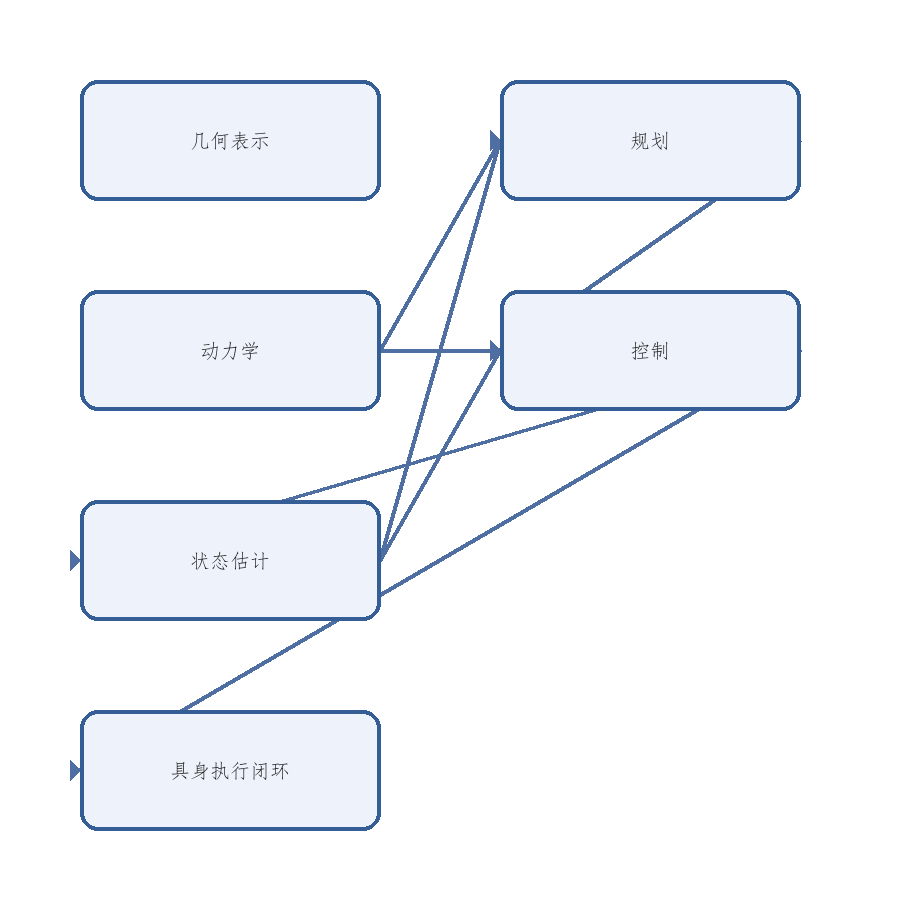
\includegraphics[width=0.9\textwidth,height=0.72\textheight,keepaspectratio]{figures/05-经典机器人学关系图.png}
\caption{05-经典机器人学关系图}
\label{fig:05-经典机器人学关系图}
\end{figure}

在当前版本中，\texttt{\detokenize{图 5-1 经典机器人学关系图}} 已承担“几何表示 - 动力学 - 规划 - 控制 - 状态估计”主关系图的职责；\texttt{\detokenize{表 5-1 经典机器人学基础与后续章节映射表}} 则把这些基础如何回流到 VLA、世界模型与部署章节正式固定下来。 本章的代码支撑重点放在两类最能代表后续具身系统接口的问题上：一类是“任务空间控制 / 阻抗控制”，用于说明高层意图如何落到可执行接触行为；另一类是 \path{EKF / 因子图状态估计}，用于说明不确定观测如何被组织成可用于控制与规划的状态变量。这样的取舍更符合本章作为基础层的职责，即用少量代表性骨架揭示核心机制，而不是把正文扩展成算法实现手册。

\section*{表 5-1 经典机器人学基础与后续章节映射表}
\addcontentsline{toc}{chapter}{表 5-1 经典机器人学基础与后续章节映射表}
\markboth{表 5-1 经典机器人学基础与后续章节映射表}{表 5-1 经典机器人学基础与后续章节映射表}

\begingroup
\small
\begin{xltabular}{\textwidth}{YYYY}
\toprule
经典基础主题 & 本章核心问题 & 在后续章节中的主要映射 & 典型关注变量 \\
\midrule
\endfirsthead
\toprule
经典基础主题 & 本章核心问题 & 在后续章节中的主要映射 & 典型关注变量 \\
\midrule
\endhead
几何表示与坐标变换 & 如何把观测、连杆、末端与环境放入统一状态空间 & 08 系统分层接口、09 感知与表征、11 VLA 输入输出接口 & 位姿、坐标系、一致性、标定误差 \\
运动学与可达性 & 某个目标在当前本体与约束下是否可执行 & 12 规划与中间表示、15 部署约束、23 场景任务分解 & 工作空间、奇异位形、逆解稳定性 \\
动力学与接触 & 执行动作时力、惯量、摩擦与冲击如何影响结果 & 10 世界模型、14 sim2real、15 硬件约束 & 质量矩阵、接触模式、摩擦、时延 \\
轨迹规划 & 如何在约束下生成可执行、可恢复的动作序列 & 12 规划推理、13 数据闭环、17 前沿专题 & 约束、平滑性、重规划代价、失败恢复 \\
闭环控制 & 如何让计划变成稳定执行，而不是离线脚本 & 11 动作表示、15 边缘部署、16 安全回退 & 带宽、稳定裕度、跟踪误差、饱和 \\
状态估计 & 如何在噪声、延迟与部分可观测下得到可信状态 & 09 多模态感知、10 内部状态、16 验证与监控 & 可观测性、协方差、漂移、同步误差 \\
建图与环境记忆 & 如何把环境结构转化为可检索、可更新的内部表示 & 07 记忆增强、10 世界模型、12 长程规划 & 拓扑、语义、时效性、可更新性 \\
约束与安全边界 & 如何给高层策略设置不可越界的物理边界 & 15 系统集成、16 安全治理、23 商业化部署 & 限幅、保护区、故障模式、接管条件 \\
\bottomrule
\end{xltabular}
\endgroup

\section*{图 5-2 接触操作的观测 - 阻抗 - 安全回退闭环}
\addcontentsline{toc}{chapter}{图 5-2 接触操作的观测 - 阻抗 - 安全回退闭环}
\markboth{图 5-2 接触操作的观测 - 阻抗 - 安全回退闭环}{图 5-2 接触操作的观测 - 阻抗 - 安全回退闭环}

\noindent\textit{源文件：\texttt{\detokenize{assets/diagrams/05-接触操作闭环图.mmd}}}
\begin{figure}[htbp]
\centering
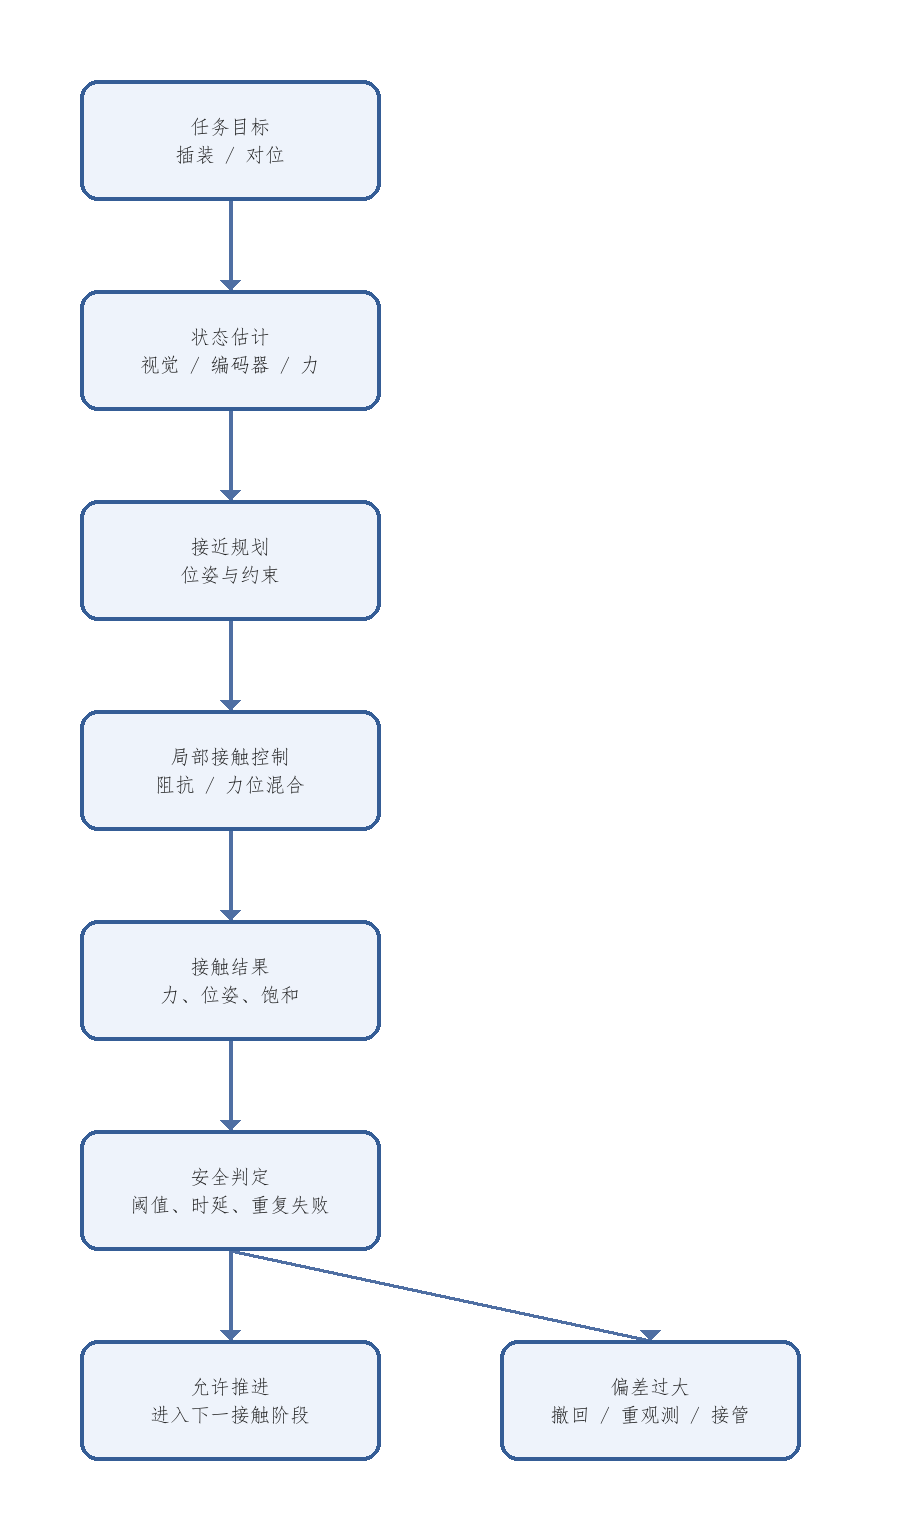
\includegraphics[width=0.9\textwidth,height=0.72\textheight,keepaspectratio]{figures/05-接触操作闭环图.png}
\caption{05-接触操作闭环图}
\label{fig:05-接触操作闭环图}
\end{figure}


\texttt{\detokenize{图 5-2}} 服务于前述柔顺插装案例：它把高层目标、状态估计、局部接触控制和安全回退分开绘制，避免把“识别到目标”误解为“已经获得可执行动作”。图中最快的安全回退通道应能绕过高层推理直接作用于局部控制；这一责任边界会在第 08、15 和 16 部分继续展开。

\section*{表 5-2 接触操作工程案例检查表}
\addcontentsline{toc}{chapter}{表 5-2 接触操作工程案例检查表}
\markboth{表 5-2 接触操作工程案例检查表}{表 5-2 接触操作工程案例检查表}

\begingroup
\small
\begin{xltabular}{\textwidth}{YYYYY}
\toprule
检查维度 & 柔顺插装中的具体问题 & 可观测证据 & 典型失效 & 推荐处理 \\
\midrule
\endfirsthead
\toprule
检查维度 & 柔顺插装中的具体问题 & 可观测证据 & 典型失效 & 推荐处理 \\
\midrule
\endhead
几何与标定 & 插头、插孔和末端坐标是否仍在同一参考系 & 重投影误差、末端位姿残差、外参版本 & 视觉定位正确但实际接触点偏移 & 重观测、标定复核、缩小接近速度 \\
接触状态 & 当前是自由运动、初触、滑动、卡滞还是已插入 & 力/力矩变化、速度下降、接触持续时间 & 把卡滞误判为正常插入 & 限力、撤回、改变接近方向 \\
局部控制 & 刚度、阻尼和位置/力通道是否与任务匹配 & 跟踪误差、接触力峰值、振荡频谱 & 刚度过高导致冲击，过低导致无法对位 & 分阶段调参、限制增益、局部搜索 \\
时间契约 & 力观测和控制命令是否仍在有效时间窗内 & 时间戳差、通信抖动、控制周期 & 过时观测驱动了新的力命令 & 丢弃过期帧、降级到保守模式 \\
安全回退 & 哪些条件必须中断自主执行 & 碰撞阈值、关节限位、重复失败计数 & 反复尝试导致过载或磨损 & 立即撤回、记录失败、请求人工接管 \\
\bottomrule
\end{xltabular}
\endgroup

\section*{代码 5-1 任务空间控制最小骨架}
\addcontentsline{toc}{chapter}{代码 5-1 任务空间控制最小骨架}
\markboth{代码 5-1 任务空间控制最小骨架}{代码 5-1 任务空间控制最小骨架}

\begin{lstlisting}[language=python]
import numpy as np

def task_space_pd(x, x_ref, J, dq, Kp, Kd):
    e = x_ref - x
    dx = J @ dq
    wrench = Kp @ e - Kd @ dx
    tau = J.T @ wrench
    return tau
\end{lstlisting}

上面的骨架只保留了一个最核心事实：高层规划最后必须通过 Jacobian、误差反馈和关节力矩映射，才能变成真实可执行的闭环命令。
